%======================================================================
\section{Capacidad, gemelo, márgenes y riesgo (F5b)}\label{sec:f5b}
%======================================================================
\paragraph{Qué se busca.} F5a.3 dejó una pregunta abierta: con la caja archivada el MPC
siempre satura, y con el actuador físico el límite de 1220~K queda lejos. En ninguno de los
dos casos una capa de riesgo puede cambiar una decisión. Esta sección recorre la ruta del
plan (§8.12--8.15) en cuatro pasos:
\begin{enumerate}
  \item ubicar la capacidad del ACS en la que el MPC tiene decisiones libres y hay riesgo;
  \item corregir lo que el gemelo no sabe: el caudal real del ACS y el pronóstico de fuga;
  \item agregar márgenes: primero deterministas (DSM) y después probabilísticos;
  \item medir todo con las métricas de la tesis y contra el PID de la tesis.
\end{enumerate}
Cambio en la planta: la capacidad del ACS (\code{acs\_max}), su rampa (\code{acs\_ramp}) y su
eficiencia $\eta$ (\code{acs\_eta}) son ahora parámetros de la réplica del HRM, y limitan por
igual a quien mueva la bomba.

%----------------------------------------------------------------------
\subsection{Paso 1: mapa de capacidad}
%----------------------------------------------------------------------
Familia extrema (14 realizaciones), $\dot m_{\max}\in\{15,\dots,70\}$~kg/s y rampas de
2.5--10~kg/s por paso; N2+sesgo frente al PI del DET con la misma capacidad y la misma $\eta$
(\code{julia/f5b1a\_capacity\_sweep.jl}).

\begin{figure}[H]\centering
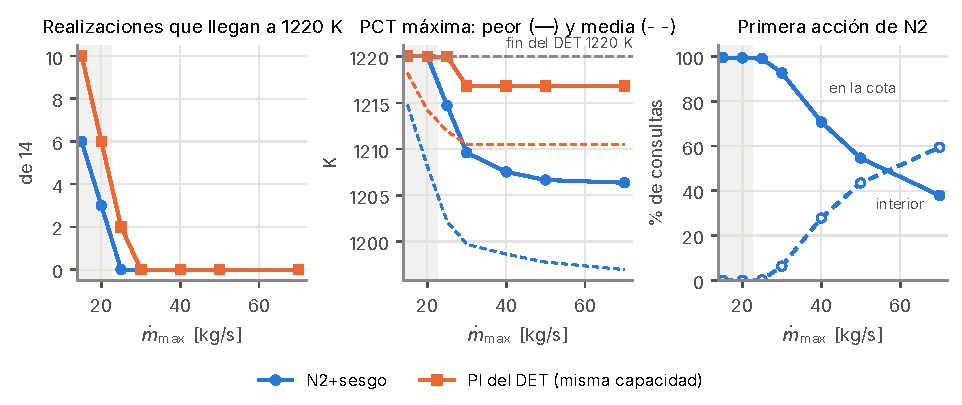
\includegraphics[width=\linewidth]{figures/fig_f5b_capacity_map.pdf}
\caption{Mapa de capacidad (rampa 5~kg/s por paso). Con $\le20$~kg/s, N2 está siempre en la
cota y llega a 1220~K en 3--6 de 14 realizaciones; el PI, en 6--10. Con $\ge40$~kg/s, N2
decide en el interior el 28--60\,\% de las veces y no hay riesgo.}
\end{figure}

\begin{figure}[H]\centering
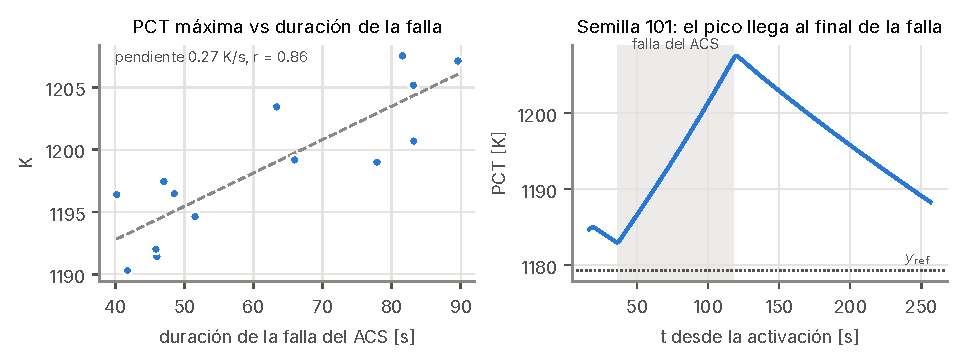
\includegraphics[width=\linewidth]{figures/fig_f5b_peak_at_failure.pdf}
\caption{De dónde sale el pico: la PCT máxima llega siempre al final de la falla del ACS, y
crece con su duración ($\approx0.3$~K/s, $r=0.86$).}
\end{figure}

\takeaway{El régimen «decisión libre y con riesgo» está vacío en la familia extrema. Donde
hay riesgo, el actuador ya está saturado; donde hay capacidad libre, las fallas de 30--90~s no
alcanzan a llevar la PCT a 1220~K. La única palanca de una capa de riesgo es pre-enfriar
antes de una falla posible.}

%----------------------------------------------------------------------
\subsection{Paso 2: lo que el gemelo no sabe}
%----------------------------------------------------------------------
\begin{itemize}
  \item \textbf{Pronóstico de fuga sin la ley de Park.} Un filtro de Kalman de tendencia
        lineal local (nivel y pendiente), con intervención ante saltos de la rotura, es 5--10
        veces más preciso que la persistencia con ruido de medición y tiene la cobertura
        calibrada (\code{python/f5b0\_leak\_forecast.py}). Sin la intervención, no se
        recupera de un salto.
  \item \textbf{En lazo cerrado no importa.} El pronosticador y el caudal medido del ACS
        cambian las decisiones (hasta 4~kg/s), pero no la PCT: las diferencias pareadas son
        $0.00\pm0.00$~K en 14 realizaciones, con y sin saltos. La inercia térmica filtra las
        diferencias de caudal y la corrección de sesgo absorbe el resto.
\end{itemize}

%----------------------------------------------------------------------
\subsection{Paso 3.i: márgenes deterministas (DSM) en la familia extrema}
%----------------------------------------------------------------------
N2+DSM con $U\in\{1244,1220\}$~K, $\tau\in\{0.00238, 0.1, 0.25\}$ y
$\lambda_s\in\{10^3,10^4,10^5\}$ no cambia la PCT máxima en más de 0.002~K. El DSM se
activa cuando la PCT predicha supera la consigna, y eso ocurre durante la falla y después de
ella, cuando N2 ya está en la cota. El PI del DET con la consigna de N2 no inyecta nada: su
margen \emph{es} su consigna de 1144~K.

%----------------------------------------------------------------------
\subsection{Paso 3.i.0: el peso del DSM, como en la tesis, frente al PID}\label{sec:dsm-lambda}
%----------------------------------------------------------------------
\paragraph{Qué se prueba.} En la tesis, con metaheurísticas (LJ), el término
$\lambda_{\rm dsm}\sum_k[\mathrm{DSM}_k-0.00238]_+^2$ con
$\mathrm{DSM}_k=(\hat y_k-y_{\rm ref})/(U-y_{\rm ref})$ \emph{sí} cambió la trayectoria cuando la
bomba tenía holgura ($u_{\max}=56.90$~A $\approx43.6$~kg/s). Con $\lambda=10^6$ sobre-enfrió
1.6~K, y $\lambda=10^4$ fue el ajuste final (\code{results/results\_penalty\_saturation},
\code{results/results\_retuned\_lambda1e4}). Aquí se repite el barrido con N2+sesgo, con
$\lambda_{\rm dsm}\in\{0,10^2,\dots,10^6\}$ y $U\in\{1244,1220\}$~K, en los mismos escenarios
de la tesis. Se compara con el PID de la tesis (\code{matlab/pid\_controller.m}: $K_p=-0.5$,
$K_i=-0.4$~A/K, consigna $y_{\rm ref}$, 56.68--100~A, 60~A/s) y con el PI interno del DET. Las
métricas son las de la tesis (\code{calculate\_performance\_metrics.m}), con una banda de 0.30~K
(\code{julia/f5b1b0\_dsm\_lambda.jl}).

\paragraph{Conjuntos.} (A) La realización archivada, con la grilla de la tesis (61 consultas
desde 1160~s) y una extendida de 241 consultas. (B) 20 realizaciones de la familia nominal,
121 consultas cada una. En ambos, bomba archivada (12.9~kg/s) o ampliada (43.6~kg/s), con
rampa blanda como en la tesis y la planta limitada a la misma capacidad. (C) 9 realizaciones de
la familia DET acelerada (semillas 201--209), a 40~kg/s y en 481 consultas. Con fallas, el
DSM tampoco cambia el pico (la PCT máxima es idéntica) y sólo agrega variación del control. El
PID duplica el IAE de N2, sube el pico 2.1~K y se asienta en 1 de 9 realizaciones.

\begin{table}[H]\centering\scriptsize\setlength{\tabcolsep}{3pt}
\begin{tabularx}{\linewidth}{@{}Y r r r r r r r r@{}}\toprule
Controlador & IAE [K$\cdot$s] & Alcanza [s] & Asienta [s] & Err.\ estac.\ [K] & Sobrepaso mín.\ [K] & PCT pico [K] & VT [kg/s] & Llegan a 1220\\ \midrule
\multicolumn{9}{@{}l}{\textit{Realización archivada, grilla de la tesis (61 consultas), bomba archivada 12.9~kg/s}}\\
N2+sesgo & 15.6 & 13.5 & 13.5 & +0.01 & -0.02 & 1181.17 & 29 & 0/1\\
N2+DSM, $\lambda$=$10^4$, $U$=1244 & 15.6 & 13.5 & 13.5 & +0.01 & -0.02 & 1181.17 & 29 & 0/1\\
N2+DSM, $\lambda$=$10^6$, $U$=1220 & 15.6 & 13.5 & 13.5 & +0.01 & -0.02 & 1181.17 & 29 & 0/1\\
PID de la tesis & 27.6 & 15.5 & $\infty$ & +1.12 & -1.47 & 1181.25 & 13 & 0/1\\
PID de la tesis, sin límite & 262.0 & $\infty$ & $\infty$ & +8.59 & -10.31 & 1181.25 & 1463 & 0/1\\
PI del DET & 88.2 & $\infty$ & $\infty$ & -3.74 & +1.94 & 1183.22 & 0 & 0/1\\
\addlinespace
\multicolumn{9}{@{}l}{\textit{Realización archivada, grilla de la tesis (61 consultas), bomba ampliada 43.6~kg/s}}\\
N2+sesgo & 3.7 & 3.0 & 3.0 & +0.01 & -0.07 & 1181.06 & 100 & 0/1\\
N2+DSM, $\lambda$=$10^4$, $U$=1244 & 3.7 & 3.0 & 3.0 & +0.01 & -0.07 & 1181.06 & 100 & 0/1\\
N2+DSM, $\lambda$=$10^6$, $U$=1220 & 3.7 & 3.0 & 3.0 & +0.01 & -0.07 & 1181.06 & 101 & 0/1\\
PID de la tesis & 99.6 & 4.5 & $\infty$ & +4.02 & -4.84 & 1181.25 & 87 & 0/1\\
PID de la tesis, sin límite & 262.0 & $\infty$ & $\infty$ & +8.59 & -10.31 & 1181.25 & 1463 & 0/1\\
PI del DET & 88.2 & $\infty$ & $\infty$ & -3.74 & +1.94 & 1183.22 & 0 & 0/1\\
\addlinespace
\multicolumn{9}{@{}l}{\textit{Familia nominal, 20 realizaciones, bomba archivada}}\\
N2+sesgo & 13.4 & 11.9 & 11.9 & +0.01 & -0.02 & 1181.00 & 30 & 0/20\\
N2+DSM, $\lambda$=$10^4$, $U$=1244 & 13.4 & 11.9 & 11.9 & +0.01 & -0.02 & 1181.00 & 30 & 0/20\\
N2+DSM, $\lambda$=$10^6$, $U$=1220 & 13.4 & 11.9 & 11.9 & +0.01 & -0.02 & 1181.00 & 30 & 0/20\\
PID de la tesis & 92.7 & 13.4 & $\infty$ & +1.89 & -2.70 & 1181.07 & 26 & 0/20\\
PID de la tesis, sin límite & 450.1 & $\infty$ & $\infty$ & +6.50 & -9.45 & 1181.07 & 1336 & 0/20\\
PI del DET & 210.9 & $\infty$ & $\infty$ & -4.92 & +1.77 & 1184.55 & 0 & 0/20\\
\addlinespace
\multicolumn{9}{@{}l}{\textit{Familia nominal, 20 realizaciones, bomba ampliada}}\\
N2+sesgo & 3.5 & 2.9 & 2.9 & +0.01 & -0.08 & 1180.89 & 99 & 0/20\\
N2+DSM, $\lambda$=$10^4$, $U$=1244 & 3.5 & 2.9 & 2.9 & +0.01 & -0.08 & 1180.89 & 99 & 0/20\\
N2+DSM, $\lambda$=$10^6$, $U$=1220 & 3.6 & 2.9 & 2.9 & +0.01 & -0.11 & 1180.89 & 98 & 0/20\\
PID de la tesis & 177.5 & 3.9 & $\infty$ & +2.26 & -4.51 & 1181.07 & 87 & 0/20\\
PID de la tesis, sin límite & 450.1 & $\infty$ & $\infty$ & +6.50 & -9.45 & 1181.07 & 1336 & 0/20\\
PI del DET & 210.9 & $\infty$ & $\infty$ & -4.92 & +1.77 & 1184.55 & 0 & 0/20\\
\addlinespace
\multicolumn{9}{@{}l}{\textit{Familia DET acelerada (con fallas), 40~kg/s (9 realizaciones)}}\\
N2+sesgo & 576.6 & 12.1 & 62.6 (2 no) & -2.61 & -0.09 & 1188.39 & 152 & 0/9\\
N2+DSM, $\lambda$=$10^4$, $U$=1244 & 576.7 & 12.1 & 62.6 (2 no) & -2.61 & -0.10 & 1188.39 & 157 & 0/9\\
N2+DSM, $\lambda$=$10^6$, $U$=1220 & 577.8 & 12.1 & 65.1 (2 no) & -2.61 & -0.34 & 1188.39 & 179 & 0/9\\
PID de la tesis & 1163.1 & 13.6 & 238.5 (8 no) & -1.31 & -7.95 & 1190.50 & 202 & 0/9\\
PI del DET & 3009.4 & 175.6 & $\infty$ & +5.80 & -15.76 & 1207.89 & 58 & 1/9\\
\bottomrule
\end{tabularx}
\caption{Métricas de la tesis (medias sobre las realizaciones). «Alcanza»: primer instante con $|e|\le0.30$~K; «Asienta»: instante desde el cual no sale de la banda ($\infty$: nunca; entre paréntesis, las realizaciones que no se asientan). Error estacionario: media de $y_{\rm ref}-\mathrm{PCT}$ en el último 20\,\%. VT: variación total del caudal entregado. Tiempos desde la primera consulta. Las demás combinaciones de $\lambda_{\rm dsm}$ y $U$ dan lo mismo que N2 (\code{results/f5b1b0\_dsm\_lambda/runs.csv}).}
\label{tab:dsm-lambda}
\end{table}


\begin{figure}[H]\centering
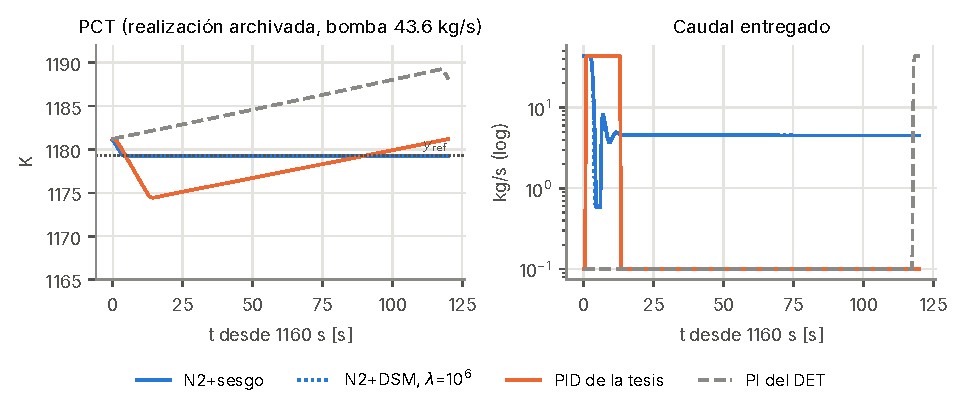
\includegraphics[width=\linewidth]{figures/fig_f5b_dsm_lambda_archived.pdf}
\caption{Realización archivada con bomba ampliada. N2 y N2+DSM ($\lambda=10^6$) son
indistinguibles: llegan a la consigna en 3~s. El PID de la tesis satura 13~s, sobre-enfría
hasta 1174.5~K y deja la bomba apagada $\sim$100~s, hasta que la PCT vuelve a pasar la
consigna. El PI del DET recién inyecta a los 118~s.}
\end{figure}

\paragraph{Por qué el DSM no mueve a N2 y sí movía al lazo de la tesis.}
\begin{enumerate}
  \item \textbf{El umbral es una banda de 0.15~K sobre la consigna.} Con $\tau=0.00238$, el
        término sólo actúa si la PCT predicha supera $y_{\rm ref}+0.15$~K. N2 resuelve su QP
        al óptimo y, con la corrección de sesgo, su predicción coincide con la planta. Por eso
        la PCT predicha queda dentro de esa banda salvo en el transitorio inicial, y ahí el
        actuador ya está en la cota (el mismo hallazgo 1 de la tesis).
  \item \textbf{En la tesis el término se activaba por razones que N2 no tiene.} LJ devolvía
        acciones subóptimas (hasta +18\,933\,\% de brecha, corregido después), y la
        predicción del lazo archivado (ROM + BiLSTM) se separaba de la planta. Cuando la
        predicción dice que la PCT sube, el DSM empuja a enfriar más: así sobre-enfrió.
  \item \textbf{Cambiar $U$ de 1244 a 1220~K} sólo reescala la banda (0.15~K pasa a
        0.10~K): no cambia nada.
\end{enumerate}

\paragraph{N2 frente al PID de la tesis.} En la tesis, el PID archivado tenía el mejor IAE
(17.8~K$\cdot$s frente a 36.5 del LJ). Su integrador había partido cargado al revés por
el artefacto de extrapolación del lazo archivado (§\ref{sec:extremos}: una caída espuria de
la PCT a 1163.5~K a los 1161~s), y eso lo mantuvo en el mínimo durante los primeros 6
pasos. En la réplica, sin el artefacto, la misma ley reacciona con toda la capacidad, ya que
su ganancia efectiva es $\approx100$~kg/s por K. Sobre-enfría y nunca se asienta en la banda
de 0.30~K. N2 llega a la consigna en 3~s (bomba ampliada) o 12~s (archivada) y queda ahí, con
un IAE entre 2 veces menor (bomba archivada, grilla de la tesis) y 50 veces menor (familia
nominal, bomba ampliada).

\takeaway{El peso del DSM no cambia la trayectoria de N2 en ningún escenario, porque N2 ya
sigue la consigna con más precisión que la banda de 0.15~K del DSM. Para que el margen actúe
hay que pedir más que «no pasar la consigna»: un umbral bajo la consigna (que equivale a
correrla) o un margen ligado a un evento, como la cota de riesgo del paso 3.ii. Frente al PID
de la tesis, N2+DSM gana en todas las métricas de la tesis.}


%----------------------------------------------------------------------
\subsection{Paso 3.ii: fallas como en el DET y una cota de riesgo}
%----------------------------------------------------------------------
\paragraph{El modelo de fallas del DET.} El ACS tiene 5 componentes en serie, y cada uno es
una cadena de Markov operativo $\leftrightarrow$ fallado, con tasas $\lambda_i$ y $\mu_i$
(\code{msfcn\_indirectps\_hrm\_c.c}, \code{MCDET\_conferencepaper\_database.mat}). Con las
tasas reales, una falla en 240~s tiene probabilidad $\approx4\cdot10^{-6}$ y dura días. Se
usa la opción acelerada que el propio modelo trae comentada ($\lambda\times10^5$,
$\mu\times10^4$): las fallas llegan a razón de $1.6\cdot10^{-3}$~s$^{-1}$ y duran según una
mezcla de exponenciales (mediana 29~s, 5.7\,\% más de 130~s). Las realizaciones se
condicionan a que haya al menos una falla en la ventana del MPC.

\begin{figure}[H]\centering
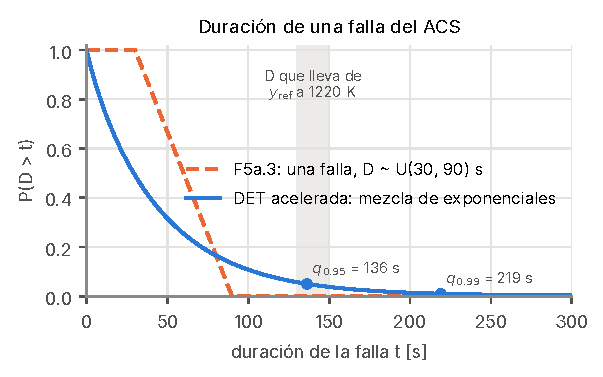
\includegraphics[width=0.62\linewidth]{figures/fig_f5b_failure_duration.pdf}
\caption{Duración de una falla. La familia extrema de F5a.3 nunca pasaba de 90~s; la del DET
tiene cola, y en esa cola está el riesgo de llegar a 1220~K.}
\end{figure}

\paragraph{La cota de riesgo.} Si el ACS falla ahora y la falla dura $q_{1-\alpha}(D)$, el ROM
predice un calentamiento $\Delta T$. N2 mantiene $\hat y_k+d\le1220-\Delta T$, con holgura
penalizada en norma $\ell_1$ exacta: sigue siendo un QP. Así
$P(\mathrm{PCT}_{\rm pico}>1220\mid\text{falla ahora})\le\alpha$.

\begin{table}[H]\centering\footnotesize\setlength{\tabcolsep}{4pt}
\begin{tabularx}{\linewidth}{@{}Y r r r r r@{}}\toprule
Caso (60 realizaciones) & Llegan a 1220~K & Peor PCT & $\Delta$ PCT máx.\ vs N2 & ISE / ISE(N2) & Masa extra\\\midrule
N2+sesgo & 0 & 1218.5~K & --- & 1.00 & ---\\
N2+cota, $\alpha=0.05$ & 0 & 1212.0~K & $-1.1\pm0.6$~K & 0.81 & +2\,\%\\
N2+cota, $\alpha=0.02$ & 0 & 1212.0~K & $-4.0\pm1.3$~K & 2.58 & +17\,\%\\
N2+cota, $\alpha=0.01$ & 0 & 1212.0~K & $-5.0\pm1.6$~K & 6.45 & +33\,\%\\
PI del DET & 7 & 1220.1~K & $+20.1\pm1.4$~K & 8.8 & +19\,\%\\\bottomrule
\end{tabularx}
\caption{Cota de riesgo con fallas como en el DET (40~kg/s, rampa 5).}
\end{table}

\begin{figure}[H]\centering
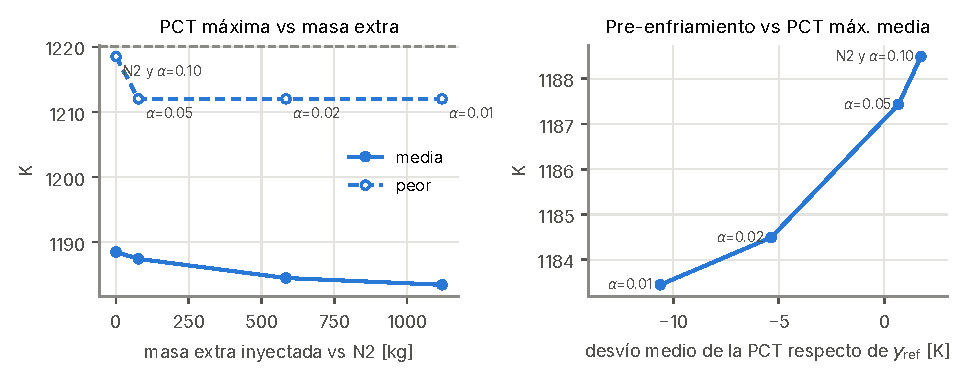
\includegraphics[width=\linewidth]{figures/fig_f5b_risk_frontier.pdf}
\caption{Frontera costo--riesgo de la cota. $\alpha=0.05$ baja la peor PCT 6.5~K y reduce el
ISE; con $\alpha\le0.02$ se paga con pre-enfriamiento.}
\end{figure}

\takeaway{Con fallas como en el DET, la cota de riesgo compra margen donde importa (la peor
realización baja de 1218.5 a 1212~K) y con $\alpha=0.05$ lo hace casi gratis. Ninguna variante
de N2 cruzó 1220~K en 60 realizaciones, así que comparar probabilidades de cruce exige un
estimador de menor varianza (plan §8.14).}
